

\tikzset{every picture/.style={line width=0.75pt}} %set default line width to 0.75pt        

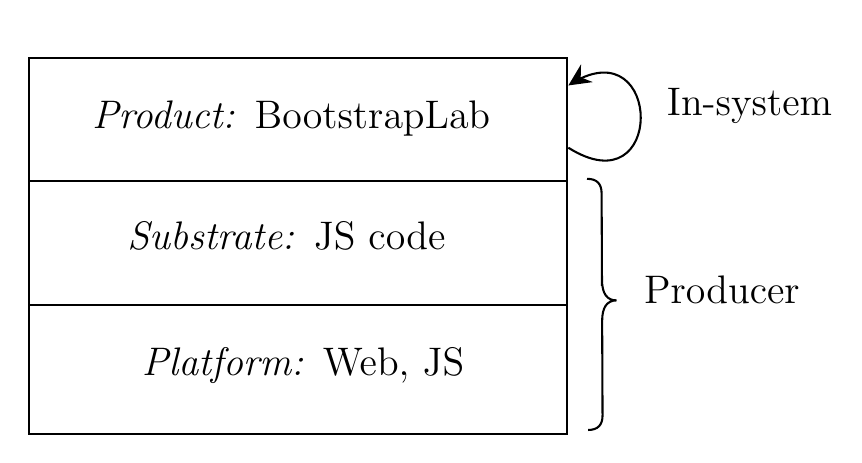
\begin{tikzpicture}[x=0.75pt,y=0.75pt,yscale=-1,xscale=1]
%uncomment if require: \path (0,228); %set diagram left start at 0, and has height of 228

%Shape: Rectangle [id:dp48332564445841997] 
\draw   (29,17) -- (288.33,17) -- (288.33,198) -- (29,198) -- cycle ;
%Straight Lines [id:da13147944738057582] 
\draw    (29,76) -- (289,76) ;
%Straight Lines [id:da013745210033387911] 
\draw    (29,136) -- (289,136) ;
%Shape: Brace [id:dp7428772270423712] 
\draw   (298.5,196) .. controls (303.17,195.98) and (305.49,193.64) .. (305.47,188.97) -- (305.28,143.59) .. controls (305.25,136.92) and (307.57,133.58) .. (312.24,133.56) .. controls (307.57,133.58) and (305.23,130.26) .. (305.2,123.59)(305.21,126.59) -- (305.02,81.97) .. controls (305,77.3) and (302.66,74.98) .. (297.99,75) ;
%Curve Lines [id:da18063245971403874] 
\draw    (289,60) .. controls (335.79,89.55) and (334.55,2.67) .. (291.02,28.73) ;
\draw [shift={(289,30)}, rotate = 326.6] [fill={rgb, 255:red, 0; green, 0; blue, 0 }  ][line width=0.08]  [draw opacity=0] (10.72,-5.15) -- (0,0) -- (10.72,5.15) -- (7.12,0) -- cycle    ;

% Text Node
\draw (82,155) node [anchor=north west][inner sep=0.75pt]  [font=\Large] [align=left] {\textit{Platform:} Web, JS};
% Text Node
\draw (75,94) node [anchor=north west][inner sep=0.75pt]  [font=\Large] [align=left] {\textit{Substrate:} JS code};
% Text Node
\draw (58,36) node [anchor=north west][inner sep=0.75pt]  [font=\Large] [align=left] {\textit{Product: }BootstrapLab};
% Text Node
\draw (324,120) node [anchor=north west][inner sep=0.75pt]  [font=\Large] [align=left] {Producer};
% Text Node
\draw (335,30) node [anchor=north west][inner sep=0.75pt]  [font=\Large] [align=left] {In-system};


\end{tikzpicture}
